\documentclass{article}
\usepackage[margin=1in]{geometry}
\usepackage{pgf}
\usepackage{tikz}
\usetikzlibrary{arrows,automata}
\usepackage[latin1]{inputenc}
\usepackage{listings}
\lstdefinestyle{customc}{
  belowcaptionskip=1\baselineskip,
  breaklines=true,
  frame=L,
  xleftmargin=\parindent,
  language=C,
  showstringspaces=false,
  basicstyle=\footnotesize\ttfamily,
  keywordstyle=\bfseries\color{green!40!black},
  commentstyle=\itshape\color{purple!40!black},
  identifierstyle=\color{blue},
  stringstyle=\color{orange},
}
\lstset{escapechar=@,style=customc}

\begin{document}

\lstinputlisting[caption=shrink\_active\_list, style=customc]{src/shrink_active_list.c}
\newpage

\begin{figure}
\center
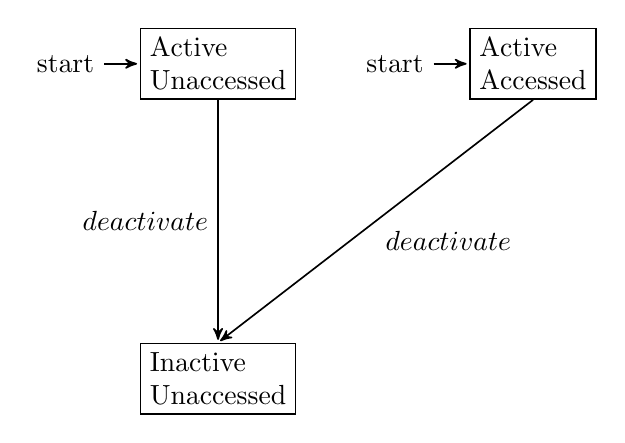
\begin{tikzpicture}[->,>=stealth',shorten >=1pt,auto,node distance=4cm,
                    semithick]

  \tikzstyle{every state}=[rectangle,draw,align=left]

  \node[state]         (IU)               {Inactive \\ Unaccessed};
  \node[initial,state] (AU) [above of=IU] {Active   \\ Unaccessed};
  \node[initial,state] (AA) [right of=AU] {Active   \\ Accessed  };

  \path
  (AU) edge [in=90,out=270,looseness=0,swap] node {$deactivate$} (IU)
  (AA) edge [in=90,out=270,looseness=0]      node {$deactivate$} (IU)
  ;

\end{tikzpicture}
\caption{Anon LRU Automata}
\end{figure}

\begin{figure}
\center
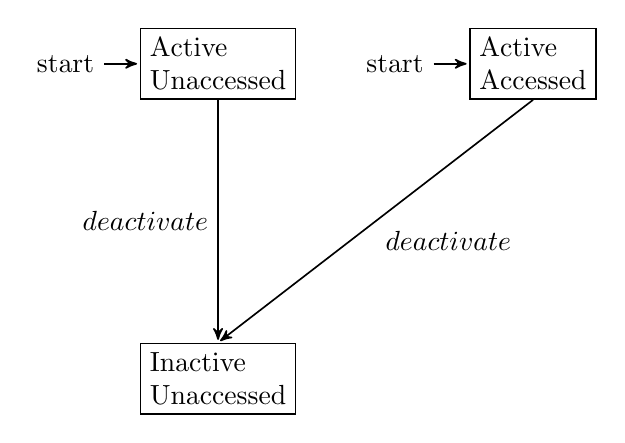
\begin{tikzpicture}[->,>=stealth',shorten >=1pt,auto,node distance=4cm,
                    semithick]

  \tikzstyle{every state}=[rectangle,draw,align=left]

  \node[state]         (IU)               {Inactive \\ Unaccessed};
  \node[initial,state] (AU) [above of=IU] {Active   \\ Unaccessed};
  \node[initial,state] (AA) [right of=AU] {Active   \\ Accessed  };

  \path
  (AU) edge [in=90,out=270,looseness=0,swap] node {$deactivate$} (IU)
  (AA) edge [in=90,out=270,looseness=0]      node {$deactivate$} (IU)
  ;
\end{tikzpicture}
\caption{File LRU Automata}
\end{figure}

\begin{figure}
\center
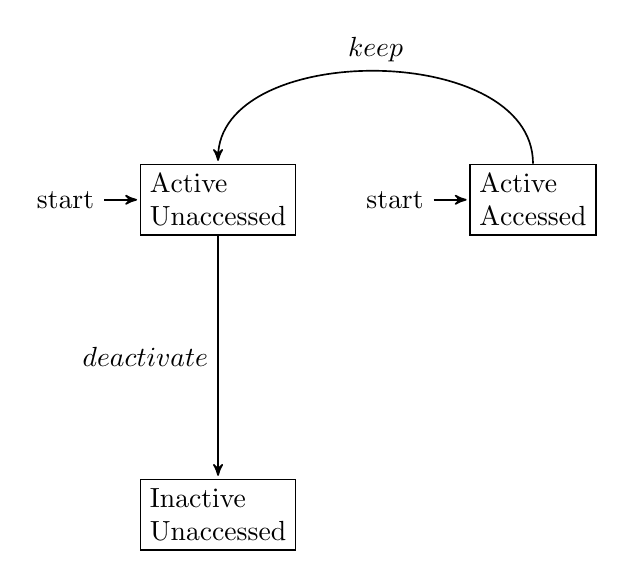
\begin{tikzpicture}[->,>=stealth',shorten >=1pt,auto,node distance=4cm,
                    semithick]

  \tikzstyle{every state}=[rectangle,draw,align=left]

  \node[state]         (IU)               {Inactive \\ Unaccessed};
  \node[initial,state] (AU) [above of=IU] {Active   \\ Unaccessed};  
  \node[initial,state] (AA) [right of=AU] {Active   \\ Accessed};

  \path
  (AA) edge [in=90,out=90,looseness=1,swap] node {$keep$} (AU)
  (AU) edge [in=90,out=270,looseness=0,swap] node {$deactivate$} (IU)
  ;
\end{tikzpicture}
\caption{VM\_EXEC File LRU Automata}
\end{figure}

\end{document}
